\documentclass{scrartcl} % scrartcl of scrreprt
% Include all project wide packages here.
\usepackage{fullpage}
\usepackage{polyglossia}
\setmainlanguage{dutch}
\usepackage{csquotes}
\usepackage{graphicx}
\usepackage{epstopdf}
\usepackage{pdfpages}
\usepackage{caption}
\usepackage[list=true]{subcaption}
\usepackage{float}
%\usepackage{mathtools}
\usepackage{standalone}
\usepackage{import}
\usepackage{tocloft}
\usepackage{wrapfig}
\usepackage{authblk}
\usepackage{array}
\usepackage{booktabs}
\usepackage[toc,page,title,titletoc]{appendix}
\usepackage{xunicode}
\usepackage{amsmath}
\usepackage{fontspec}
\usepackage{unicode-math}
\usepackage[
    backend=bibtexu,
	texencoding=utf8,
bibencoding=utf8,
    style=ieee,
    sortlocale=nl_NL,
    language=auto
]{biblatex}
\usepackage{listings}
\newcommand{\includecode}[3][c]{\lstinputlisting[caption=#2, escapechar=, style=#1]{#3}}
\newcommand{\superscript}[1]{\ensuremath{^{\textrm{#1}}}}
\newcommand{\subscript}[1]{\ensuremath{_{\textrm{#1}}}}


\newcommand{\chapternumber}{\thechapter}
\renewcommand{\appendixname}{Bijlage}
\renewcommand{\appendixtocname}{Bijlagen}
\renewcommand{\appendixpagename}{Bijlagen}

\usepackage[hidelinks]{hyperref} %<--------ALTIJD ALS LAATSTE

\renewcommand{\familydefault}{\sfdefault}

\setmainfont[Ligatures=TeX]{Myriad Pro}
\setmathfont{Asana Math}
\setmonofont{Lucida Console}

\usepackage{titlesec, blindtext, color}
\definecolor{gray75}{gray}{0.75}
\newcommand{\hsp}{\hspace{20pt}}
\titleformat{\chapter}[hang]{\Huge\bfseries}{\chapternumber\hsp\textcolor{gray75}{|}\hsp}{0pt}{\Huge\bfseries}
\renewcommand{\familydefault}{\sfdefault}
\renewcommand{\arraystretch}{1.2}
\setlength\parindent{0pt}

%For code listings
\definecolor{black}{rgb}{0,0,0}
\definecolor{browntags}{rgb}{0.65,0.1,0.1}
\definecolor{bluestrings}{rgb}{0,0,1}
\definecolor{graycomments}{rgb}{0.4,0.4,0.4}
\definecolor{redkeywords}{rgb}{1,0,0}
\definecolor{bluekeywords}{rgb}{0.13,0.13,0.8}
\definecolor{greencomments}{rgb}{0,0.5,0}
\definecolor{redstrings}{rgb}{0.9,0,0}
\definecolor{purpleidentifiers}{rgb}{0.01,0,0.01}


\lstdefinestyle{csharp}{
language=[Sharp]C,
showspaces=false,
showtabs=false,
breaklines=true,
showstringspaces=false,
breakatwhitespace=true,
escapeinside={(*@}{@*)},
columns=fullflexible,
commentstyle=\color{greencomments},
keywordstyle=\color{bluekeywords}\bfseries,
stringstyle=\color{redstrings},
identifierstyle=\color{purpleidentifiers},
basicstyle=\ttfamily\small}

\lstdefinestyle{c}{
language=C,
showspaces=false,
showtabs=false,
breaklines=true,
showstringspaces=false,
breakatwhitespace=true,
escapeinside={(*@}{@*)},
columns=fullflexible,
commentstyle=\color{greencomments},
keywordstyle=\color{bluekeywords}\bfseries,
stringstyle=\color{bluestrings},
identifierstyle=\color{purpleidentifiers}
}

\lstdefinestyle{vhdl}{
language=VHDL,
showspaces=false,
showtabs=false,
breaklines=true,
showstringspaces=false,
breakatwhitespace=true,
escapeinside={(*@}{@*)},
columns=fullflexible,
commentstyle=\color{greencomments},
keywordstyle=\color{bluekeywords}\bfseries,
stringstyle=\color{redstrings},
identifierstyle=\color{purpleidentifiers}
}

\lstdefinestyle{xaml}{
language=XML,
showspaces=false,
showtabs=false,
breaklines=true,
showstringspaces=false,
breakatwhitespace=true,
escapeinside={(*@}{@*)},
columns=fullflexible,
commentstyle=\color{greencomments},
keywordstyle=\color{redkeywords},
stringstyle=\color{bluestrings},
tagstyle=\color{browntags},
morestring=[b]",
  morecomment=[s]{<?}{?>},
  morekeywords={xmlns,version,typex:AsyncRecords,x:Arguments,x:Boolean,x:Byte,x:Char,x:Class,x:ClassAttributes,x:ClassModifier,x:Code,x:ConnectionId,x:Decimal,x:Double,x:FactoryMethod,x:FieldModifier,x:Int16,x:Int32,x:Int64,x:Key,x:Members,x:Name,x:Object,x:Property,x:Shared,x:Single,x:String,x:Subclass,x:SynchronousMode,x:TimeSpan,x:TypeArguments,x:Uid,x:Uri,x:XData,Grid.Column,Grid.ColumnSpan,Click,ClipToBounds,Content,DropDownOpened,FontSize,Foreground,Header,Height,HorizontalAlignment,HorizontalContentAlignment,IsCancel,IsDefault,IsEnabled,IsSelected,Margin,MinHeight,MinWidth,Padding,SnapsToDevicePixels,Target,TextWrapping,Title,VerticalAlignment,VerticalContentAlignment,Width,WindowStartupLocation,Binding,Mode,OneWay,xmlns:x}
}

%defaults
\lstset{
basicstyle=\ttfamily\small,
extendedchars=false,
numbers=left,
numberstyle=\ttfamily\tiny,
stepnumber=1,
tabsize=4,
numbersep=5pt
}
\addbibresource{../../library/bibliography.bib}

\author{}
\title{EPO3: Eindrapport - Decoder}

\begin{document}
\chapter{Ontwerpspecificaties van de GPU}
\label{ch:spec}

\section {Functie van de GPU}
Een GPU is geïntegreerde schakeling, ontworpen om aan de hand van ingangsdata bepaalde vormen op een beeldscherm te tekenen, zodat een bruikbaar beeld ontstaat. De GPU moet dit met een dusdanige frequentie kunnen, dat de wijzigingen aan het beeld vloeiend overkomen op het menselijk oog en het beeld niet knippert. De GPU die voor dit project ontworpen en gefabriceerd wordt, zal een sterk versimpelde versie zijn van de GPU's die vandaag de dag in consumentenelektronica te vinden zijn.
\\\\
De GPU is ontworpen volgens het blokschema in figuur~\ref{fig:spec-overzicht} aan het einde van dit hoofdstuk.
Zoals er in het blokschemate zien is, is er randapparatuur nodig om de GPU een afbeelding op een monitor te laten schrijven. Ten eerste is er een CPU met zijn eigen RAM nodig, om de benodigde data (instructies) voor een enkel frame te sturen naar de GPU. De GPU moet deze data omzetten naar een verzameling pixels en deze in een screen buffer in het externe SRAM schrijven. Er wordt gebruik gemaakt van twee screen buffers, zodat het huidige frame niet wordt overschreven met de data van het volgende frame. Ook moet de GPU het huidige frame van de screenbuffer uit het SRAM kunnen uitlezen, om deze vervolgens te om te zetten naar een signaal dat door een VGA monitor verwerkt kan worden tot een schermafbeelding. Dit externe SRAM is nodig, omdat er op de chip zelf niet genoeg transistoren aanwezig zijn om een VRAM te maken met de grootte die benodigd is om twee screen buffers op te kunnen slaan.

%Aanpassen deze figuur
\begin{figure}[H]
\centering
	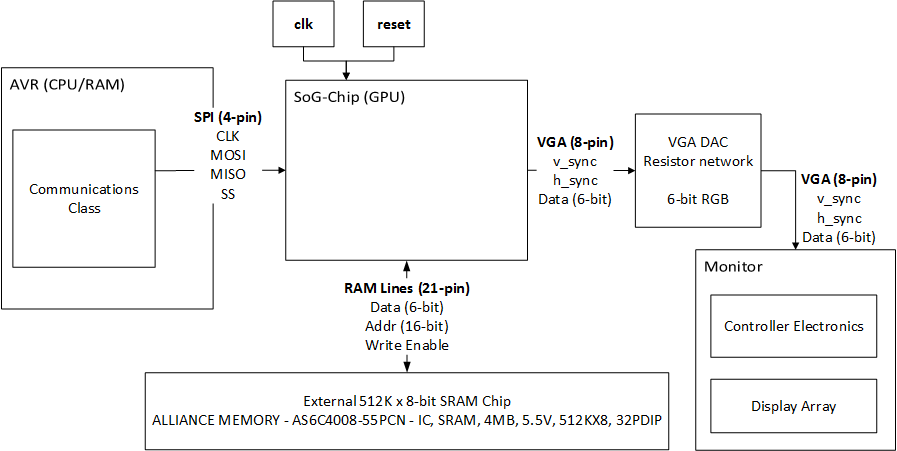
\includegraphics[scale=0.9]{Resource/system_overview.png}
	\caption{Een systematisch overzicht van de GPU}
	\label{fig:spec-overzicht}
\end{figure} 


\section{Specificaties}
Om een GPU van acceptabel niveau te ontwerpen, zijn de volgende functionele eisen gesteld:

\begin{itemize}
	\item De GPU wordt aangestuurd door een externe CPU
	\item De GPU maakt gebruikt van extern SRAM als VRAM (videogeheugen)
	\item De GPU moet in staat zijn om een aantal elementaire vormen (pixels, vierkanten en lijnen) en sprites op een beeldscherm te tekenen.
	\item De GPU krijgt data betreffende deze elementaire vormen vanuit de CPU (een AVR), bijvoorbeeld voor een vierkant bestaat de data uit de x- en y-coördinaten, breedte, hoogte en kleur
	\item De communicatie tussen de CPU en de GPU wordt door een SPI-interface verzorgd
	\item Het beeldscherm wordt aangestuurd middels een VGA-signaal, wat gegenereerd wordt door de GPU
	\item De GPU ondersteunt een beeldschermresolutie van 160 bij 120 pixels, met een kleurdiepte van 6 bits (64 individuele kleuren)
	\item De communicatie tussen het externe VRAM en de GPU wordt met een parallelle bus (6 bist data, 16 bits adres) tot stand gebracht
\end{itemize}

\section {Randvoorwaarden van de IC}

De bij dit project ontworpen chip wordt uitgevoerd met de Sea-of-Gates techniek. Dit houdt in dat er een vast aantal transistoren, pinnen en oppervlak beschikbaar wordt gesteld. Het is zaak dit aantal zo goed mogelijk te benutten voor een optimaal resultaat. Door deze voorwaarde moet bij het ontwerp rekening gehouden worden met een aantal randvoorwaarden/ontwerpeisen. Deze randvoorwaarden zijn gegeven in de projecthandleiding en hieronder voor de volledigheid nog eens opgesomd. \cite{epo3-manual}

\begin{itemize}
\item Voor schakelingen van het type FSM (Finite State Machine) mag alleen een synchroon (Moore)-type gebruikt worden
worden
\item Als de schakeling geactiveerd wordt, moeten alle FSM’s in hun resettoestand komen door middel van een resetsignaal
\item Voor het genereren van het kloksignaal kan gebruik gemaakt worden van een kristal van 6.144 MHz of 32 kHz, dat extern wordt aangesloten aan de IC met 2 pinnen
\item Het kristal voor de klok wordt met 2 pinnen aangesloten aan de IC en heeft een klokfrequentie is 6.144 Mhz
\item Het streven is om zo weinig mogelijk componenten extern te gebruiken. De dissipatie van de chip dient echter ook beperkt te zijn. Dit geeft een compromis voor de maximale stroom
die de elektronica mag dissiperen voor de aansturing van de LEDs, etc.
\item De voedingsspanning van het IC bedraagt 5 Volt
\item Het IC wordt gemaakt met een 1.6 µm nwell-CMOS proces (het Philips C3DM proces)
\item Het beschikbare chip-oppervlak is circa $0.4  cm^2$ , hetgeen overeenkomt met ongeveer 40.000 transistorparen, die gelijk zijn verdeeld over 2 bond bars
\item Er zijn op het IC 36 verbonden aansluitingen, waarvan vier pinnen voor de voeding zijn, twee voor het kloksignaal en nog eens één voor het reset-signaal
\end {itemize}

\textbf{Parameters Sea-of-Gates}
\begin {itemize}
\item $V_{DD} = 5V$
\item$ V_{T0} = 0.7V$
\item  $t_{ox} = 25 ∗ 10^{−9}m$
\item Nmos L×W = 1.6 × 23.2µm
\item Pmos L×W = 1.6 × 29.6µm
\end {itemize}


\end{document}
